\documentclass[tikz,border=10pt]{standalone}
\usepackage{pgfplots, amsmath}
\pgfplotsset{compat=1.17}
\usetikzlibrary{calc, arrows, positioning, shapes.geometric, backgrounds, patterns}
\usepgfplotslibrary{fillbetween, groupplots}
\begin{document}

% Q1
\begin{tikzpicture}
\begin{axis}[
    xlabel={$t \text{ (s)}$},
    ylabel={$v \text{ (ms}^{-1}\text{)}$},
    axis lines=middle,
    grid=none,
    xmin=0, xmax=14,
    ymin=0, ymax=25,
    xtick={0,5,13},
    ytick={0,2,22},
    xticklabels={$0$, $5$, $13$},
    yticklabels={$0$, $2$, $22$},
    xlabel style={at={(axis description cs:1,0)},anchor=west},
    ylabel style={at={(axis description cs:0,1)},anchor=south},
    width=12cm, height=6cm,
    every axis plot/.append style={very thick},
]
\addplot[black] coordinates {(0,2) (5,22) (13,22)};
\addplot[dashed] coordinates {(5,0) (5,22)};
\addplot[dashed] coordinates {(13,0) (13,22)};
\addplot[dashed] coordinates {(0,22) (5,22)};
\end{axis}
\node at (0,-0.5) {$O$};  % Add this line to place the origin label
\end{tikzpicture}

% Q1 (solution)
\begin{tikzpicture}
\begin{axis}[
    xlabel={$t \text{ (s)}$},
    ylabel={$v \text{ (ms}^{-1}\text{)}$},
    axis lines=middle,
    grid=none,
    xmin=0, xmax=14,
    ymin=0, ymax=25,
    xtick={0,5,13},
    ytick={0,2,22},
    xticklabels={$0$, $5$, $13$},
    yticklabels={$0$, $2$, $22$},
    xlabel style={at={(axis description cs:1,0)},anchor=west},
    ylabel style={at={(axis description cs:0,1)},anchor=south},
    width=12cm, height=6cm,
    every axis plot/.append style={very thick},
]
\addplot[black] coordinates {(0,2) (5,22) (13,22)};
\addplot[dashed] coordinates {(0,2) (5,2)};
\addplot[dashed] coordinates {(5,0) (5,22)};
\addplot[dashed] coordinates {(13,0) (13,22)};
\addplot[dashed] coordinates {(0,22) (5,22)};
\end{axis}
\node at (0,-0.5) {$O$};  % Add this line to place the origin label
\end{tikzpicture}

% Q2
\begin{tikzpicture}
\begin{axis}[
    xlabel={$t \text{ (m)}$},
    ylabel={$v \text{ (ms}^{-1}\text{)}$},
    axis lines=middle,
    grid=none,
    xmin=0, xmax=8,
    ymin=0, ymax=6,
    xtick={0,3,7},
    ytick={0,5},
    xticklabels={$0$, $5$, $40\text{m } 54\text{s}$},
    yticklabels={$0$, $x$},
    xlabel style={at={(axis description cs:1,0)},anchor=west},
    ylabel style={at={(axis description cs:0,1)},anchor=south},
    width=12cm, height=6cm,
    every axis plot/.append style={very thick},
]
\addplot[black] coordinates {(0,0) (3,5) (7,5)};
\addplot[dashed] coordinates {(3,0) (3,5)};
\addplot[dashed] coordinates {(7,0) (7,5)};
\addplot[dashed] coordinates {(0,5) (3,5)};
\end{axis}
\node at (0,-0.5) {$O$};  % Add this line to place the origin label
\end{tikzpicture}

% Q3
\begin{tikzpicture}
\begin{axis}[
    xlabel={$t \text{ (s)}$},
    ylabel={$v \text{ (ms}^{-1}\text{)}$},
    axis lines=middle,
    grid=none,
    xmin=0, xmax=200,
    ymin=0, ymax=30,
    xtick={0,60,120,190},
    ytick={0,25},
    xticklabels={$0$, $60$, $120$, $T$},
    yticklabels={$0$, $25$},
    xlabel style={at={(axis description cs:1,0)},anchor=west},
    ylabel style={at={(axis description cs:0,1)},anchor=south},
    width=12cm, height=6cm,
    every axis plot/.append style={very thick},
]
\addplot[black] coordinates {(0,0) (60,25) (120,25) (190,0)};
\addplot[dashed] coordinates {(0,25) (60,25)};
\addplot[dashed] coordinates {(60,25) (60,0)};
\addplot[dashed] coordinates {(120,25) (120,0)};
\end{axis}
\node at (0,-0.5) {$O$};  % Add this line to place the origin label
\end{tikzpicture}

% Q4
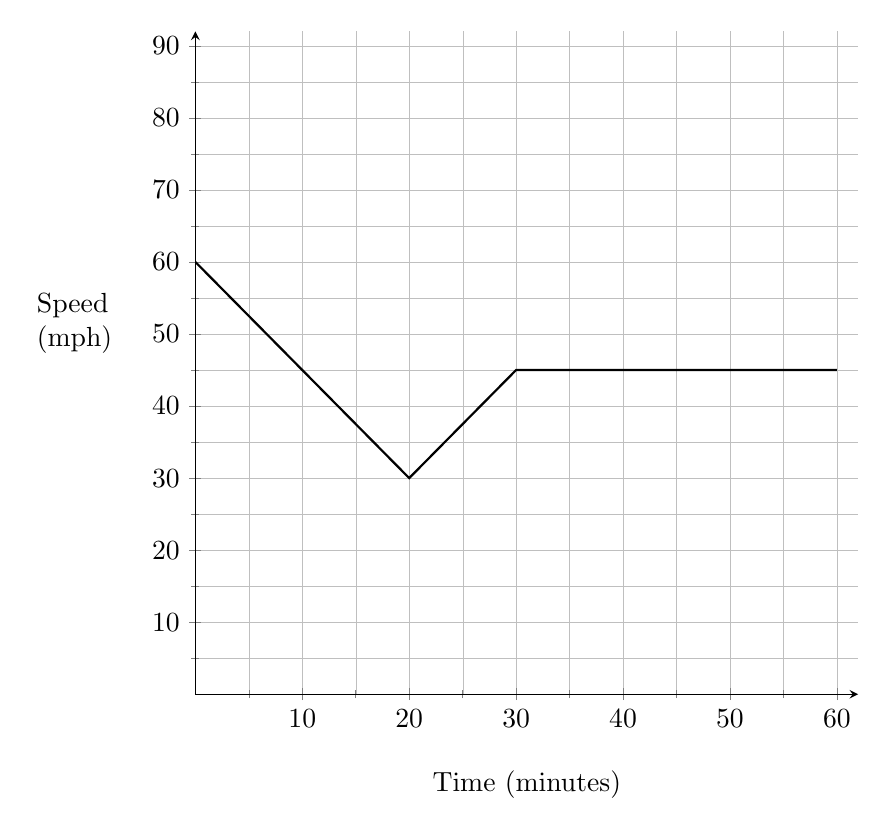
\begin{tikzpicture}
\begin{axis}[
    xlabel={Time (minutes)},
    ylabel={\parbox{1.5cm}{Speed (mph)}},
    axis lines=middle,
    grid=both,
    grid style={line width=.1pt, draw=gray!50},
    major grid style={line width=.2pt, draw=gray!50},
    minor tick num=1,
    xmin=0,
    xmax=62,
    ymin=0,
    ymax=92,
    xtick={0,10,20,30,40,50,60},
    xticklabels={0,10, 20, 30, 40, 50, 60},
    ytick={0,10,20,30,40,50,60, 70, 80, 90},
    xlabel style={at={(axis description cs:0.5,-0.1)},anchor=north},
    ylabel style={at={(axis description cs:-0.15,0.5)},anchor=south},
    width=10cm,
    height=10cm,
]
\addplot[thick, black] coordinates {(0,60) (20,30) (30,45) (60, 45)};
\end{axis}
\end{tikzpicture}

\end{document}
